\documentclass{pnu-survey}

%%%%%%%%%%%%%%%%%%%%%%%%%%%%%%%%%%%%%%%%%%%%%%%
% 필요한 패키지가 있다면 하단에 적어주세요.
%%%%%%%%%%%%%%%%%%%%%%%%%%%%%%%%%%%%%%%%%%%%%%%
% 이미지 및 그래프 관련 패키지
\usepackage{graphicx}
\usepackage{float}
\usepackage{subfloat}
\usepackage{subfigure}
\usepackage{lscape}
\usepackage{enumitem}

% \usepackage[compact]{titlesec}

% 수학 기호 관련
\usepackage{gensymb}
\usepackage{amsmath}
\usepackage{amssymb}
\usepackage{amsthm}
\usepackage{exscale}
\usepackage{textcomp}

\newcommand{\cl}[1]{\textcircled{\scriptsize #1}}

% 알고리즘 표현
\usepackage{algorithmic}
\usepackage{algorithm}

% customize algorithmic environment
\renewcommand{\algorithmicrequire}{\makebox[40px]{\hfill\textbf{Input :}}}
\renewcommand{\algorithmicensure}{\makebox[40px]{\hfill\textbf{Output :}}}

% 테이블 관련
\usepackage{array}
\usepackage{tabulary}
\usepackage{multirow}
\usepackage[table]{xcolor}
\usepackage{ctable}
\usepackage{booktabs}

% 미주 표현
\usepackage{endnotes}
\renewcommand\notesname {참고 사이트}

% 제목, 저자, 요약
\title{Big-Tech기업을 중심으로 알아보는 컴퓨터 전공자의 2022 - 2023 취업 동향}
\author{손재성(son73097@pusan.ac.kr)}
\abstract{
Big-Tech에 관한 정의나, Big-Tech로 분류되는 기업에는 다양한 의견이 존재한다. 본 논문에서는  "빅테크의 공정한 규제 방향에 관한 연구"~\cite{ksb}에서 제시한 Big-Tech 기업의 개념을 만족하는 기업을 Big-Tech 기업으로 서술할 것이다. 본 논문에서는 한국의 Big-Tech 기업으로 여겨지는 "네카라쿠배" 를 중심으로 컴퓨터 전공자의 2023년 취업 동향에 대해 분석한다.
}

\begin{document}

\maketitle

\section{서론}

Big-Tech 기업은 AI, 전자 상거래, 온라인 광고, 소비자용 전자 제품, 클라우드 컴퓨팅, 컴퓨터 소프트웨어, 미디어 스트리밍, 스마트 홈, 자율 주행 자동차, SNS와 같은 다양한 기술 영역에서 해당 영역의 플랫폼을 기반으로 막대한 사용자를 보유한 기업이다. Big-Tech는 원래 미국의 거대 IT기업인 Alphabet(Google), Amazon, Apple, Meta(Facebook)을 지칭하는 말로 쓰였으나, 시장지배력을 가진 온라인 플랫폼을 기반으로 디지털 서비스를 제공하는 기업까지 확대하여 사용되기도 한다. 한국에서는 소위 "네카라쿠배" 즉, NAVER, Kakao, Line, Coupang, 우아한형제들(배달의민족)이 Big-Tech기업으로 여겨진다.

본 논문에서는 비록 원래 Big-Tech로 여겨지는 회사들과 비교하여 객관적인 규모는 현저히 떨어지지만, 한국 IT업계를 대표하는 "네카라쿠배"의 2022 - 2023년 취업 동향에 대해 분석한다. 2022년 11월 기준으로 채용과 관련한 전공, 경력, 학력에 따른 채용 공고의 분석을 통해 2022 - 2023년의 컴퓨터 전공자의 취업 동향에 대해 알아볼 것이다. 마지막으로 컴퓨터 전공자가 지원할 수 있는 채용 공고에 대한 세부 직무 분류를 통해 채용 현황을 분석한다.

\section{본론}

\subsection{각 회사별 채용 현황}
각 기업의 채용 공고 사이트를 조사하여 채용 현황에 대해 분석하고 이를 바탕으로 2023년 채용 동향을 예측한다. 각 기업의 구체적인 공고별 모집 인원에 관해서는 공개되지 않았으므로, 다소의 오차가 있더라도 채용 공고의 숫자를 모집 인원으로 확대 해석하였다.

\subsubsection{NAVER}
NAVER의 경우 NAVER Careers 사이트를 이용하여 채용 공고를 조사하였다.\endnote{NAVER Careers, 2022.11 avaliable, https://recruit.navercorp.com/main.do} NAVER는 2022년 11월 기준 총 111개의 분야에 대한 채용을 진행하고 있다. 이 중 Tech분야에서는 71개의 공고가, 디자인 분야에서는 3개의 공고가, 서비스 분야에서는 30개의 공고가, 기업 경영 분야에서는 7개의 공고가 있었다. 컴퓨터 전공을 바탕으로 지원 가능한 Tech분야의 공고 71개 중에서 경력사항을 모집 요건으로 하는 "경력직" 채용은 68개였다. 입사 경험이 없는 사람을 대상으로 하는 "신입" 채용의 경우 3개의 채용이 있었다. 3개의 신입 채용은 모두 인턴쉽 형태였으며, 학사 학력으로 지원 가능한 채용은 단 1개가 있었다. 나머지 2개의 신입 채용은 석/박사 학력 소지자를 대상으로 하는 상시모집형 인턴 채용이었다. 이는 2022년 11월 7일 기준으로 진행중인 공고에 관한 사항이다. 2022년 전체로 범위를 늘이면 학사 학력으로 지원 가능한 신입 공개채용은 2개를 추가하여 총 3개, 석사 이상은 총 5개의 신입 공개 채용에 지원 가능했다. 경력직 채용의 경우 각 채용별로 월간 채용을 통해 상시모집형으로 채용이 이루어지고 있었으며, 경력의 최소 요건은 관련분야 1년이상 근무였다.

\subsubsection{Kakao}
Kakao의 경우 Kakao 영입 사이트를 이용하여 채용 공고를 조사했다.\endnote{Kakao 영입, 2022.11 available, https://careers.kakao.com/index} Kakao는 2022년 11월 기준 219개의 분야에 대한 채용을 진행하고 있다. 분야별로는 테크 134개, 서비스비즈 49개, 디자인/브랜드 18개, 스태프 18개의 채용을 진행중이다. 컴퓨터 전공을 바탕으로 지원 가능한 테크 분야의 공고 134개 중 유경력자를 대상으로 하는 경력 채용의 경우 115개, 신입도 지원 가능한 채용의 경우 19개가 존재했다. Kakao의 경우 신입 채용을 따로 진행하는데, 신입 채용으로 따로 명시하지 않은 경우 3개월간의 계약직 수습 기간을 통해 정규직으로 최종 채용한다. Kakao는 NAVER와 달리 석사, 박사 학위를 경력으로 인정한다. 따라서 학력에 따른 채용 지원 가능 여부는 별도로 조사하지 않았다. NAVER와의 공통점으로 Kakao는 경력 채용에 관한 채용 공고를 상시모집형으로 운용한다는 점이 있다.

\subsubsection{Line}
Line의 경우 LINE CAREERS 사이트를 이용하여 채용 공고를 조사했다.\endnote{LINE CAREERS, 2022.11 available, https://careers.linecorp.com/ko/} Line의 경우 한국, 일본, 태국, 대만 등 다양한 국가에 지부를 두고 있는 만큼 회사 위치가 한국인 경우만으로 조사했다. Design 카테고리에서 34개, Product planning 33개, Businisss \& Sales 20개, Corporate 19개, Marketing \& Comms 5개, Engineering 108개, 도합 총 219개의 채용 공고를 확인했다(중복 포함). 이 중 컴퓨터 전공을 바탕으로 지원 가능한 Engineering의 채용 공고 108개에서 신입 공개 채용 1개를 제외한 107개가 경력자를 대상으로 한 수시 모집이었다. Line의 경우 석사/박사 학위의 소지를 지원 조건으로 설정한 공고는 없었다. 다만 NAVER, Kakao는 경력으로 최소 1년 많게는 3년을 요구한 반면 Line의 경우 대부분 3년 많게는 5년이상의 경력을 요구하였다.

\subsubsection{Coupang}
Coupang의 경우 Coupang Careers 사이트를 이용하여 조사를 진행했다.\endnote{Coupang Careers, 2022.11 available, https://www.coupang.jobs/kr/} 물류 플랫폼을 기반으로 한 회사인 만큼, 앞선 NAVER, Kakao, Line과 같이 통신, 네트워크 서비스 플랫폼을 기반으로 한 기업에 비해 컴퓨터 전공자 이외에도 다양한 전공에서 채용을 진행함을 확인했다. 총 44개의 채용 공고에서 11개가 컴퓨터 전공자가 지원 가능한 공고였다. Coupang의 경우에도 앞선 회사들의 사례와 마찬가지로 신입 개발자 채용이 아닌 경우 수시 모집 형태로 개발자를 상시 채용중에 있었다. Coupang의 경력 모집의 경우 앞선 회사의 사례와 비교하여 매우 높은 경력을 요구했다. 최소 5년, 많게는 10년 이상의 경력을 지원 조건으로 설정했다. Line과 마찬가지로 경력을 우선시하였으므로 석사/박사 학위자를 대상으로 한 특별채용은 없었다.

\subsubsection{우아한형제들}
우아한형제들의 경우 우아한형제들 인재영입 사이트를 이용하여 조사를 진행했다.\endnote{우아한형재들 인재영입, 2022.11 available, https://career.woowahan.com/} 현재 진행 중인 채용 공고는 개발 63, PM 14, 콘텐츠/서비스 14, 영업/MD 6, 경영지원 61이었으며, 컴퓨터 전공자가 지원 가능한 개발 카테고리의 채용 63개 모두가 경력자를 대상으로 한 상시모집형 수시 채용 공고였다. 각 채용 공고마다 달랐지만 석사/박사 학력 소지자 또는 5년 이상의 실무 경력을 가진 사람을 우대하였다. 

\subsection{개발직군 요구사항/세부전공}

앞서 살펴본 한국의 Big-Tech로 여겨지는 5개 기업의 채용에서 요구되는 전공, 학력, 경력사항을 표 1과 같이 정리할 수 있다. 표1에서 ratio는 전체 채용 중 컴퓨터 전공자가 지원 가능한 직군의 비율이다. degree는 해당 분야의 경력이 없을 경우 수시 모집 채용에서 요구되는 평균 학위이다. 이때 신입 공개 채용에서 요구되는 학위는 제외하였으며, 수시 모집 시 요구되는 학위이다. 신입 공개 채용에 있어서는 모든 회사가 학사 이상의 경우 별도의 채용 과정을 통해 채용하는 형태를 띄고 있다. 상시지원형 수시 모집에서 회사 별로 채용 시 요구되는 학력은 각 수시 모집 채용 공고 별로 다소의 차이가 있었으나 대체로 같은 회사에서 요구되는 학위는 표1과 같았다. experience는 경력 채용 전형에서 요구되는 평균 경력이다. 이 역시 각 채용 공고 별로 다소 차이가 있으나 같은 회사에서 요구되는 수준은 표1 범위에 속했다.

\begin{table}[!pt]
\centering
\setlength{\belowcaptionskip}{5pt}
\caption{전공, 학력, 경력에 따른 지원 가능 채용 공고}
\label{tab:datasets}
\begin{tabular}{@{}lrrrr@{}} 
\toprule
{\bfseries Corporation} & $ratio$ & $degree$ & $experience$ \\
\midrule
NAVER			&64\%	    &석/박사	    & 2-3 year\\
Kakao   		&61.1\%		&제한없음	& 1-3 year\\
Line    		&49.3\%   	&제한없음	& 3-5 year\\
Coupang			&25\%     	&박사      	&5-10 year\\
우아한형제들		&39.9\%		&석/박사    	&   5 year\\
\bottomrule
\end{tabular}
\end{table}

그림 1은 컴퓨터 전공자의 Big-Tech채용 시 분류되는 세부 직군의 분포이다. 컴퓨터 전공자에게 요구되는 세부 직군은 매우 다양하고, 기업마다 요구되는 세부 직군은 모두 상이하다. 이를 고려하여 정보보안, 서버/백엔드, 프론트엔드, DB, AI/ML직군으로 크게 다섯 가지 세부 직군으로 분류하였다. 그림1은 앞선 절에서 설명한 5개의 회사들의 세부 전공별 직무들에 대한 채용 공고의 개수를 합산하여 그래프로 나타내어 비교한 것이다. 앞서 설명한 것처럼 각 기업마다 요구하는 세부 직군에는 다소 차이가 있다. 따라서 그림1에 포함되지 않은 세부 직무도 다수 존재한다. 또한 기업에 따라 채용하는 인원 수의 비율의 차이 역시 존재한다. 하지만 이직이 잦은 업계 특성, Big-Tech채용 현황이라는 본 논문의 주제를 고려했을 때 그림 1의 분류는 적절하다고 판단된다.

\begin{figure}[hb]
\centering
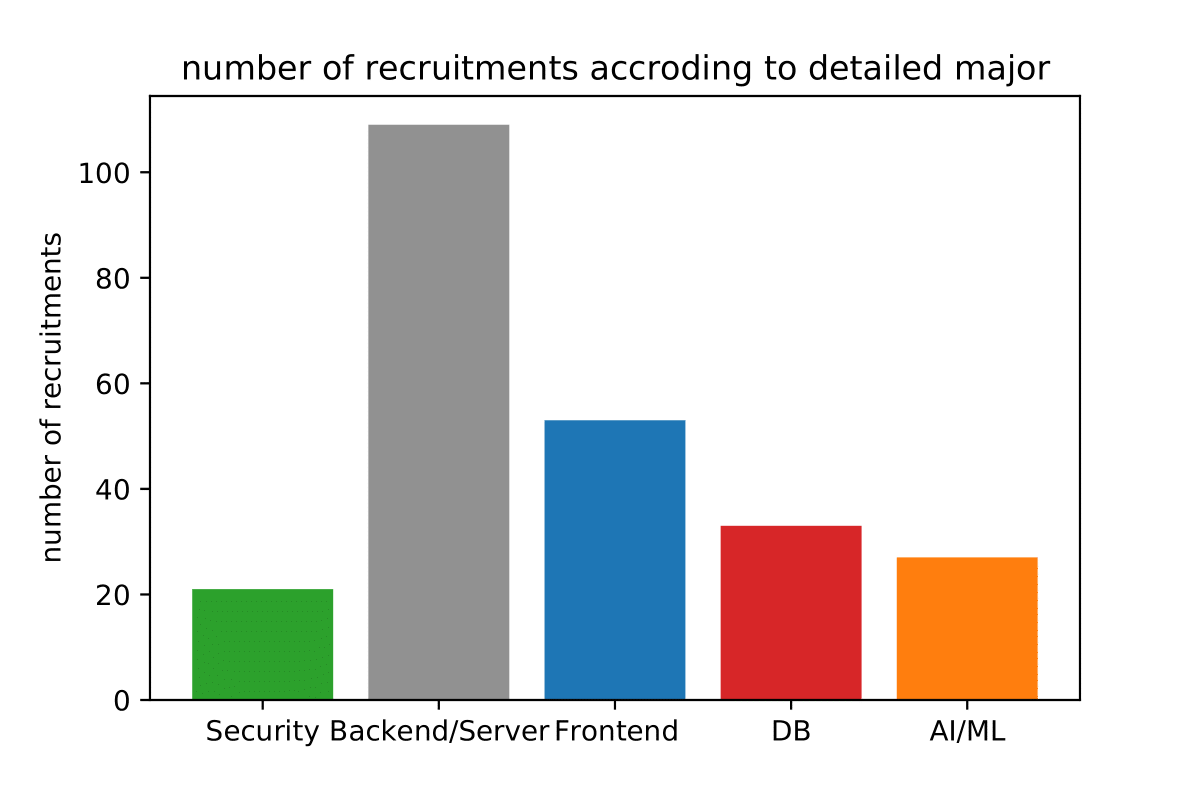
\includegraphics[width=0.4\textwidth]{img/fig1.png}
\caption{세부 직무별 채용 공고 수}
\label{fig:example1}
\end{figure}
\index{figure}

\section{결론}

 컴퓨터 전공자와 타 전공자에 따른 Big-Tech 채용 현황을 중점으로 관찰했을 때, Big-Tech로 여겨지는 "네카라쿠배"의 채용 공고에 따르면 컴퓨터 전공자를 대상으로 한 채용 공고가 적게는 25\%(Coupang) 많게는 64\%(NAVER)에 달한다. 이는 컴퓨터 전공자의 경우 타 전공자에 비해 Big-Tech로의 취업문이 비교적 크게 열려 있다는 것을 의미한다.

 최종학위에 따른 채용 현황을 중점으로 관찰했을 때, 각 회사별로 다소 차이가 있는 것을 확인했다. NAVER의 경우 석/박사 학위 소지자를 경력직으로 대우하는 Coupang, 우아한형제들과 다르게 "학위 소지 신입 채용" 으로 별도로 분류하여 채용한다. Kakao, Line의 경우 각 채용별로 다소 차이가 있지만, 대부분의 경우 학위 취득 여부를 채용 과정에 직접적으로 반영하지 않았다. 그 대신 경력을 더 중시하여 채용을 진행하는 성향을 띄었다. Coupang의 박사학위 소지자를 5년 경력급으로 대우한다는 점이 특징이었다. 석사학위 소지자와 학부 졸업생 간의 차이는 채용 공고에서는 따로 명시되지 않았다. 우아한형제들의 경우 석/박사 학위소지를 경력으로 인정하여 채용을 진행하였다.

경력사항에 따른 채용 현황을 중점으로 관찰했을 때 신입과 경력의 경우가 크게 다른 것이 특징이다. 신입 개발자의 취업 경로는 신입 채용으로 한정되어 있는 것에 반해 경력이 있는 경우 본 논문에서 언급한 다섯 개의 회사만 하더라도 각 화사별로 적게는 수십 개에서 많개는 수백 개에 달하는 상시모집형 채용을 통해 이직이 가능함을 확인할 수 있다. 각 기업에서 요구하는 경력의 정도가 다른 것 또한 특징이다. Kakao, NAVER의 경우 경력 모집에서 요구되는 경력이 대부분 3년 정도였으나, Line의 경우 3년-5년으로 이보다 다소 많은 경력을 요구했다. 우아한현제들의 경우 5년 이상의 경력을 요구하는 경우가 대부분이었고, Coupang의 경우 대부분 5년-10년의 높은 경력을 요구했다.

세부 전공에 따른 채용 현황을 관찰했을 때 Backend/Server직무의 수요가 가장 많았으며, Frontend, DB, AI/ML, 정보보안이 그 뒤를 이었다. 이는 Big-Tech기업들이 각각의 기술 플랫폼을 기반으로 사용자를 확보하고 서비스를 제공하는 운영 방식에 따른 것이라고 생각된다. 이직의 기회가 많은 업계 특성을 고려한다면 세부 전공의 선택으로 인한 채용의 폭이 크게 달라질 것임을 알 수 있다.

\bibliographystyle{ieeetr}
\bibliography{ref}
\theendnotes{}
\end{document}
